\documentclass{article}
% translate with >> pdflatex -shell-escape <file>

% This file is used as unit test for pgfplots, copyright by Christian Feuersaenger.
% 
% See
%   http://pgfplots.sourceforge.net/pgfplots.pdf
% for pgfplots.
%
% Any required input files (for <plot table> or <plot file> or the table package) can be downloaded
% at
% http://www.ctan.org/tex-archive/graphics/pgf/contrib/pgfplots/doc/latex/
% and
% http://www.ctan.org/tex-archive/graphics/pgf/contrib/pgfplots/doc/latex/plotdata/

\usepackage{pgfplots}
\pgfplotsset{compat=newest}

\pagestyle{empty}

\begin{document}

	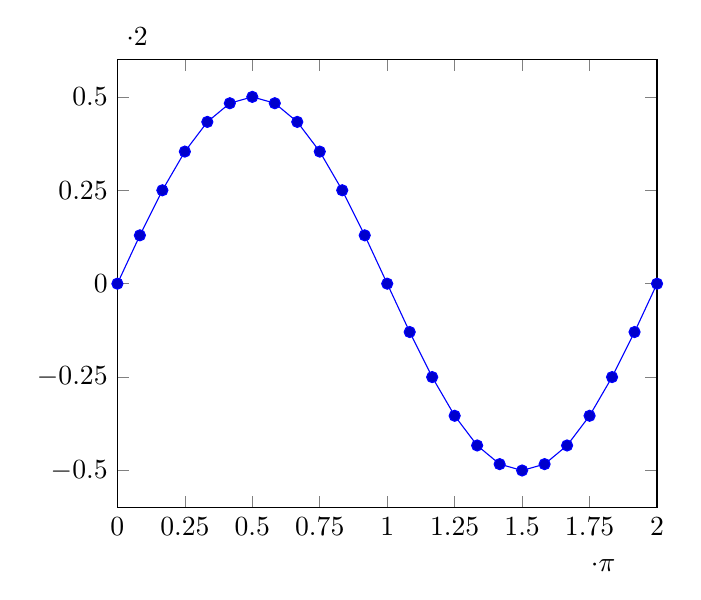
\begin{tikzpicture}
		\begin{axis}[xtick={0,0.78539,...,10},domain=0:2*pi,enlarge x limits=0,scaled x ticks={real:3.1415},xtick scale label code/.code={$\cdot \pi$},
			scaled y ticks={real:2},
		]
		\addplot (\x,{sin(\x r)});
		\end{axis}
	\end{tikzpicture}
\end{document}
